\documentclass[a4paper,12pt]{article}
\usepackage[utf8]{inputenc}
\usepackage[english]{babel}
\usepackage{graphicx}
\usepackage{amsmath}
\usepackage{amssymb}
\usepackage{hyperref}
\usepackage{geometry}
\usepackage{tabularx}
\usepackage{float}
\usepackage[backend=biber, style=numeric, sorting=none]{biblatex}
\usepackage{booktabs}
\usepackage{colortbl}
\usepackage{xcolor}
\usepackage{caption} % For customizing captions


% Set the caption font size
\captionsetup{font=small}


\addbibresource{references.bib}

\geometry{a4paper, left=25mm, right=25mm, top=25mm, bottom=25mm}
\title{Project 1: Supervised Learning - Classification}
\author{Alexander Svarfdal Gudmundsson \and Jan Babin}
\date{\today}

\begin{document}

\maketitle

\section{Introduction}
\subsection{Background}
Diabetes is a chronic condition characterised by elevated blood sugar levels. While genetic factors 
can play a role, a significant amount of diabetes Type 2 cases is associated with lifestyle choices. 
According to the World Health Organization \cite{WHO2016}, 422 million people worldwide 
are living with diabetes, with numbers continuing to rise. The societal impact of diabetes is 
significant: a diminished quality of life and a higher risk of serious health complications which in 
turn may lead to increased healthcare costs. Therefore, there is medical merit in
early predictions of diabetes to refine treatment and management strategies.

\subsection{Objective}
The goal of this project is to build a machine learning model that can identify 
patterns in lifestyle and demographic data associated with diabetes and thereby predict whether
a given person has diabetes / is very likely do develop it. While the 
model is purely intended for academic purpose, the project allows us to 
explore how machine learning can be used to analyse health-related data and 
provide insights into potential risk factors.

\subsection{Dataset}
The dataset at hand, "Diabetes, Hypertension and Stroke Prediction," is from \href{https://www.kaggle.com/datasets/prosperchuks/health-dataset/data}{Kaggle} and contains 
health-related data in CSV format intended for predicting diabetes, hypertension and stroke. 
For this project, we are solely focussing on diabetes. The dataset consists of 70,692 observations 
and 18 features, some of which are outlined as follows (for a full overview, see Table \ref{tab:feature_list} in the Appendix):
\begin{itemize}
    \item \textbf{Age}: Coded in 13 age groups (see Figure \ref{fig:age_groups}).
    \item \textbf{Sex}: Binary variable representing male (0.0) and female (1.0).
    \item \textbf{BMI}: Body Mass Index, a continuous variable.
    \item \textbf{Lifestyle indicators}: Such as smoking status (whether the individual has smoked 
    at least 100 cigarettes in their lifetime), physical activity in the past 30 days 
    (excluding job-related activity), daily fruit and vegetable consumption, and heavy alcohol 
    consumption (based on defined weekly limits for men and women).
    \item \textbf{General health and mental/physical health}: Self-reported general health on a 
    scale from 1 (excellent) to 5 (poor), along with the number of days with poor mental and 
    physical health over the past 30 days.
    \item \textbf{Pre-existing conditions}: Information on high cholesterol, coronary heart 
    disease or myocardial infarction, and difficulty walking.
\end{itemize}

\begin{figure}[h!]
    \centering
    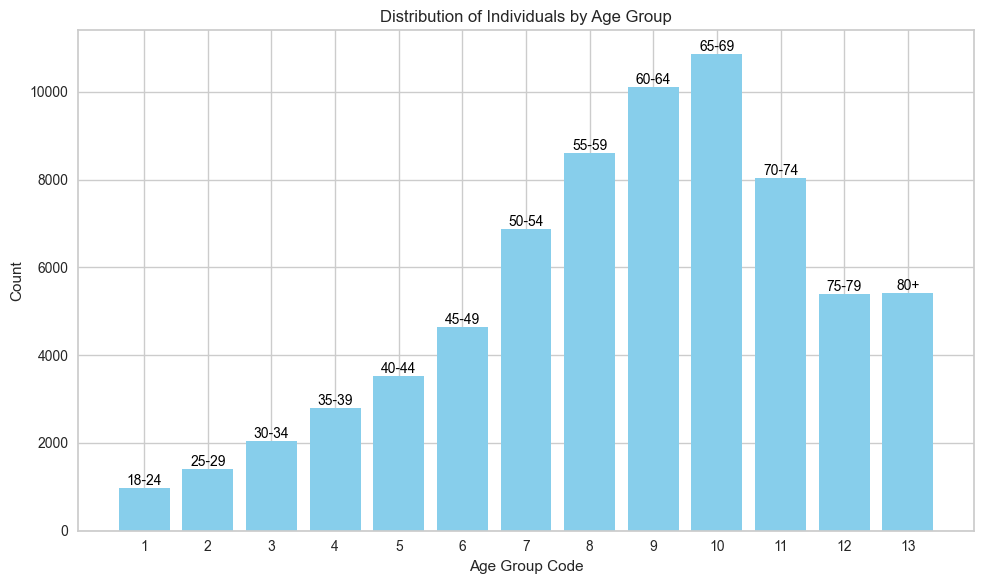
\includegraphics[width=0.7\textwidth]{plot_age_groups.png}
    \caption{Distribution of Age Groups in the Dataset: Counts of individuals across thirteen defined age groups, 
    ranging from 18 to 24 years to 80 years and older, according to the AGEG5YR scheme.}
    \label{fig:age_groups}
\end{figure}

The target variable is \textit{Diabetes}, which is represented as a binary category 
(0.0 for no diabetes, 1.0 for diabetes). No missing or null values were identified in the dataset, 
ensuring that data cleaning was minimal and straightforward. Furthermore, the dataset is perfectly 
balanced, in that, 50\% of observations correspond to diabetes, the other 50\% do not.


\section{Process}
The steps involved in the analysis follow a standard supervised machine learning pipeline, 
from data preparation to model selection and evaluation.

\section{CHECK FOR HIGH COLESTEROL AND DIABETES, part of EDA.}

\subsection{Data Loading and Exploration}
The dataset was loaded into a pandas DataFrame. Initial exploration was conducted to understand 
the structure of the data:
\begin{itemize}
    \item Data Integrity: We confirmed that the dataset contained no missing or null values.
    \item Feature Exploration: The features were analysed for their unique values and data 
    types, revealing that many variables were binary, and the rest were either categorical or 
    continuous. Continuous variables included features like \textit{BMI}, \textit{Age}, \textit{MentHlth}, 
    and \textit{PhysHlth}, while categorical variables included \textit{GenHlth} 
    (self-reported health scale from 1 to 5) and binary indicators for lifestyle factors like 
    smoking, physical activity, and alcohol consumption.
\end{itemize}

\subsection{Preprocessing}
\subsubsection{One-Hot Encoding}
Since the data set's features were numeric, we tried one-hot encoding features that seemed categorical
into binary columns to prevent the model from interpreting these as continuous data, where actually
the distance between values might not bear any meaning. 


\subsubsection{Scaling}
Certain features with a wide range of values were standardized using sklearn's \texttt{StandardScaler}. These included:
\textit{BMI}, \textit{MentHlth}, \textit{PhysHlth}, and \textit{Age}: Standardization ensures that the models 
(e.g., logistic regression, support vector machines) are not biased towards features with larger 
numeric ranges. This is important for algorithms that rely on the magnitude of features during 
decision-making.

\subsubsection{Train-Test Split}
The dataset was split into a training set (80\%) and a test set (20\%) using \texttt{train\_test\_split} from 
sklearn. We decided on this split for our relatively large data set in order to retrieve both substantial 
training and test set sizes. This reduces overfitting (model has enough training to learn nuances without 
memorising specific instances) as well as yielding a robust set of unseen data for testing and is a common industry practice. 
Stratification was applied to ensure that the class distribution of the target variable 
(\textit{Diabetes}) remained balanced across the training and test sets.

\subsection{Feature Correlation Analysis}
To explore potential multicollinearity among features, a correlation matrix was generated and
visualised using Seaborn's \texttt{heatmap} function. The goal was to identify highly correlated features 
that could negatively impact model performance by redundancy. We utilised pandas' inbuilt correlation
function that by default calculates the Pearson correlation coefficient, which is a measure of linear correlation.

\subsection{Model Selection and Evaluation}
\subsubsection{PyCaret Experiment Setup}
For model selection, we utilised PyCaret's \texttt{ClassificationExperiment} to quickly get a 
comparison between multiple classification models. The \texttt{ClassificationExperiment} tries 
different models to rank the models based on accuracy, using default hyperparameters based on common practices. 
We then selected the 5 best performing models to fine-tune further via hyperparameter optimisation. 
\\
PyCaret’s built-in random grid-search was used to tune the hyperparameters of the selected models, 
optimising for accuracy. The random grid-search works by 
randomly choosing a parameter value from a given (or a default) range. It then tries out different combinations
of these random hyperparameters and chooses the best one based on accuracy.
\\
ADD SOMETHING ABOUT CROSS VALIDATION HERE (which should be performed by the ClassifciationExperiment)


\subsubsection{Feature Selection}
Some rudimentary feature selection was employed, using PyCaret's \texttt{ClassificationExperiment}'s inbuilt
feature selection parameter. This reduces the set of features, the model is trained on, to only those deemed 
important based on statistical tests and feature importance techniques, which may help improve model 
performance.

\subsubsection{Model Stacking and Ensembling}
In an effort to improve prediction accuracy, two ensemble learning methods were applied:
\begin{itemize}
    \item A hard voting ensemble (that is, majority vote) was created that involved 
    the 5 top-performing models chosen previously, using PyCaret's \texttt{(blend\_models)}. 
    The resulting blended model runs its base models on an input
    and will output whatever was predicted most often among these.
    \item Furthermore, a combined model using stacking was also built. 
    Stacking works by training a model to aggregate the predictions of all of the predictors in a more
    sophisticated way than blending.
\end{itemize} 

\section{Results}
SOME SORT OF INTRODUCTION NEEDS TO GO HERE I GUESS - WE COULD BRIEFLY EXPLAIN THE SCORES WE PAID ATTENTION TO,
THAT IS, ACCURACY, F1, ...

\subsection{Preprocessing}
One-hot encoding features, that were already binary but numerical did not make any difference in the model's
performance. This goes to show that a model can be trained on binary features equivalently well, regardless
of whether they are represented by float or boolean values. However, one-hot encoding the 5-category-feature
\textit{GenHlth} resulted in slightly higher accuracy values for all models evaluated by \texttt{ClassificationExperiment}.
Therefore, we proceded with this encoding.
\\
Scaling continuous attributes actually resulted in some of the best models performing worse then without.
We also learnt that \texttt{ClassificationExperiment} takes care of preprocessing steps (involving scaling)
as needed for different models. Hence, we chose to omit manual scaling and let PyCaret take care of it.

\subsection{Feature Correlation Analysis}
The features \textit{GenHlth\_5.0} and \textit{PhysHlth} exhibited strong linear correlation ($r = 0.52 > 0.5$),
albeit on the lower end. Omitting \textit{GenHlth\_5.0}, however, decreased accuracy across our top 5 models,
implying the degree of correlation was not high enough to outweigh having more features / data to train 
on.

\begin{figure}[H]
    \centering
    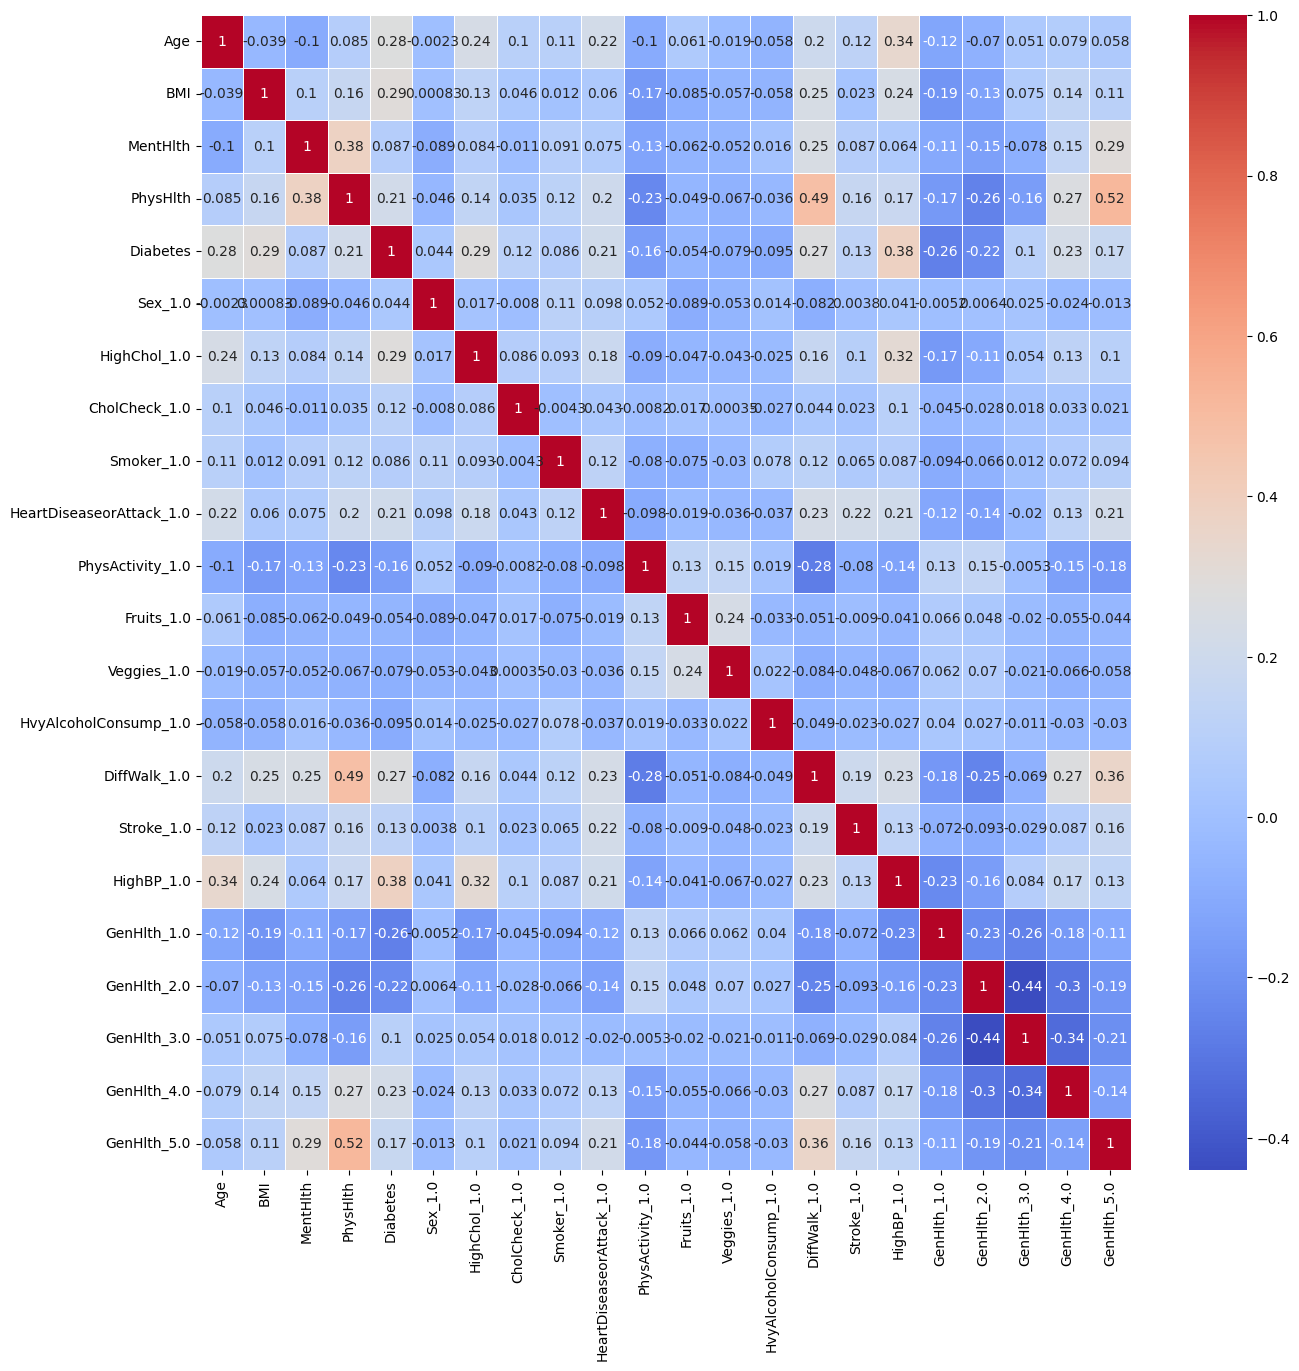
\includegraphics[width=0.7\textwidth]{correlation_matrix.png}
    \caption{Correlation matrix showing relationships between features in the dataset (Pearson correlation). 
    Higher values indicate stronger correlations.}
    \label{fig:correlation_matrix}
\end{figure}

\subsection{ClassificationExperiment}
With this setup, PyCaret's \texttt{ClassificationExperiment} yielded the following results:

\begin{table}[H]
\centering
\begin{tabular}{l l c c c c}
\toprule
\textbf{Model} & \textbf{Classifier} & \textbf{Accuracy} & \textbf{Recall} & \textbf{Precision} & \textbf{F1} \\
\midrule
\texttt{gbc} & Gradient Boosting Classifier & \cellcolor{yellow}0.7508 & 0.7897 & 0.7329 & \cellcolor{yellow}0.7601 \\
\texttt{lightgbm} & Light Gradient Boosting Machine & 0.7495 & \cellcolor{yellow}0.7926 & 0.7298 & 0.7598 \\
\texttt{ada} & Ada Boost Classifier & 0.7482 & 0.7731 & \cellcolor{yellow}0.7366 & 0.7543 \\
\texttt{lr} & Logistic Regression & 0.7467 & 0.7737 & 0.7342 & 0.7534 \\
\texttt{ridge} & Ridge Classifier & 0.7467 & 0.7799 & 0.7314 & 0.7549 \\
\texttt{lda} & Linear Discriminant Analysis & 0.7467 & 0.7798 & 0.7314 & 0.7548 \\
\texttt{rf} & Random Forest Classifier & 0.7273 & 0.7627 & 0.7124 & 0.7366 \\
\texttt{nb} & Naive Bayes & 0.7246 & 0.7251 & 0.7244 & 0.7247 \\
\texttt{et} & Extra Trees Classifier & 0.7108 & 0.7330 & 0.7019 & 0.7171 \\
\texttt{knn} & K Neighbors Classifier & 0.7019 & 0.7196 & 0.6951 & 0.7071 \\
\bottomrule
\end{tabular}
\caption{Performance of Top 10 Models after (sorted by accuracy, top scores [Accuracy, Recall, Precision, F1] highlighted)}
\label{tab:model_performance}
\end{table}

Our rudimentary feature selection analysis produced the following results:

\begin{table}[H]
    \centering
    \begin{tabular}{l l c c c c}
    \toprule
    \textbf{Model} & \textbf{Classifier} & \textbf{Accuracy} & \textbf{Recall} & \textbf{Precision} & \textbf{F1} \\
    \midrule
    \texttt{gbc} & Gradient Boosting Classifier & \cellcolor{yellow}0.7302 & \cellcolor{yellow}0.7761 & 0.7109 & \cellcolor{yellow}0.7420 \\
    \texttt{lightgbm} & Light Gradient Boosting Machine & 0.7302 & 0.7700 & 0.7133 & 0.7405 \\
    \texttt{ada} & Ada Boost Classifier & 0.7299 & 0.7581 & 0.7178 & 0.7373 \\
    \texttt{lr} & Logistic Regression & 0.7260 & 0.7350 & \cellcolor{yellow}0.7222 & 0.7284 \\
    \texttt{ridge} & Ridge Classifier & 0.7258 & 0.7374 & 0.7209 & 0.7290 \\
    \texttt{lda} & Linear Discriminant Analysis & 0.7258 & 0.7374 & 0.7209 & 0.7290 \\
    \texttt{qda} & Quadratic Discriminant Analysis & 0.7250 & 0.7514 & 0.7139 & 0.7321 \\
    \texttt{nb} & Naive Bayes & 0.7238 & 0.7382 & 0.7177 & 0.7277 \\
    \texttt{rf} & Random Forest Classifier & 0.7231 & 0.7645 & 0.7062 & 0.7341 \\
    \texttt{et} & Extra Trees Classifier & 0.7229 & 0.7530 & 0.7104 & 0.7310 \\
    \bottomrule
    \end{tabular}
    \caption{Performance of Top 10 Models after feature selection (sorted by accuracy, top scores [Accuracy, Recall, Precision, F1] highlighted)}
    \label{tab:model_performance_fs}
\end{table}
    
As can be seen, feature selection affected the best performing models negatively, we therefore 
proceeded keeping all features in the data.
After optimising the hyperparameters, the resulting scores of the five best models were as shown
(note that most models did not benefit from hyperparameter tuning): 

\begin{table}[H]
\centering
\begin{tabular}{l l c c c c}
\toprule
\textbf{Model} & \textbf{Classifier} & \textbf{Accuracy} & \textbf{Recall} & \textbf{Precision} & \textbf{F1} \\
\midrule
\texttt{lightgbm} & Light Gradient Boosting Machine & \cellcolor{yellow}0.7515 & \cellcolor{yellow}0.7930 & 0.7336 & \cellcolor{yellow}0.7603 \\  % Tuned selected based on accuracy
\texttt{gbc}    & Gradient Boosting Classifier & 0.7508 & 0.7897 & 0.7329 & 0.7601 \\  % Original selected based on accuracy
\texttt{lr}     & Logistic Regression & 0.7499 & 0.7737 & 0.7342 & 0.7534 \\  % Tuned selected based on accuracy
\texttt{ada}    & Ada Boost Classifier & 0.7482 & 0.7731 & \cellcolor{yellow}0.7366 & 0.7543 \\  % Original selected based on accuracy
\texttt{ridge}  & Ridge Classifier & 0.7467 & 0.7799 & 0.7314 & 0.7549 \\  % Original selected based on accuracy
\bottomrule
\end{tabular}
\caption{WE NEED TO CHECK IF THIS IS RIGHT Best Results of Top 5 Models (sorted by accuracy, top scores highlighted)}
\label{tab:best_model_performance}
\end{table}


\subsection{Model Stacking and Ensembling}

We ensembled the 5 best tuned models using blending:

\begin{table}[H]
    \centering
    \begin{tabular}{l c c c c}
    \toprule
    \textbf{Model} & \textbf{Accuracy} & \textbf{Recall} & \textbf{Precision} & \textbf{F1} \\
    \midrule
    \texttt{Blended Model} & 0.7495 & 0.7783 & 0.7359 & 0.7565 \\
    \bottomrule
    \end{tabular}
    \caption{Blending Results (Mean Performance Metrics)}
    \label{tab:blending_performance}
\end{table}

The scores suggest that this ensemble would perform worse than a Light Gradient Boosting model alone.
Our stacking ensemble yielded the following results:

\begin{table}[H]
    \centering
    \begin{tabular}{l c c c c}
    \toprule
    \textbf{Model} & \textbf{Accuracy} & \textbf{Recall} & \textbf{Precision} & \textbf{F1} \\
    \midrule
    \texttt{Stacking Ensemble} & 0.7500 & 0.7810 & 0.7356 & 0.7575 \\
    \bottomrule
    \end{tabular}
    \caption{Stacking Ensemble Results (Mean Performance Metrics)}
    \label{tab:stacking_performance}
\end{table}
    
Hence, a Light Gradient Boosting model would outperform a stacking ensemble, too.
Since our 5 best models included models that were based on a similar method (e.g., Light Gradient Boosting 
and Gradient Boosting), we then tried to ensemble hand-picked models in an effort to diversify the set of
base models, that is, avoid near-perfect correlation between models. We therefore selected Gradient Boosting Classifier, 
Ada Boost Classifier and Ridge Classifier (WHY DID WE NOT USE THE TUNED ONES, Light Gradient performed better).
Blending performed better than stacking, the results are shown below:

\begin{table}[H]
    \centering
    \begin{tabular}{l c c c c}
    \toprule
    \textbf{Model} & \textbf{Accuracy} & \textbf{Recall} & \textbf{Precision} & \textbf{F1} \\
    \midrule
    \texttt{Blending Ensemble} & 0.7523 & 0.7818 & 0.7383 & 0.7594 \\
    \bottomrule
    \end{tabular}
    \caption{Blending Ensemble Results with selected base models (Mean Performance Metrics)}
    \label{tab:blending_performance_handpicked}
\end{table}

This was the best model we could find for our data.


\subsection{Testing the Models with the Test Data}

After training the ensemble model on the training dataset, the model was evaluated on both the 
training and test data to measure its performance and generalization capability. 
Table \ref{tab:accuracy_results} shows the accuracy results for both the training and test sets.

\begin{table}[h]
    \centering
    \begin{tabular}{|c|c|}
        \hline
        \textbf{Dataset} & \textbf{Accuracy} \\
        \hline
        Training Data & 0.7534 \\
        Test Data & 0.7492 \\
        \hline
    \end{tabular}
    \caption{Accuracy of the ensemble model on training and test data.}
    \label{tab:accuracy_results}
\end{table}

The results indicate that the blended ensamble performs well both on the training and the test data. Since there is little to no difference between the training and the test accuracy it means that the model is able to generalize well on never seen data. 
Overfitting means that the model is learning the training data too closely, whitch is not the case in our model.
The final test accuracy of 74.92\% is the best that we could do for this project. 
Further improvement could possible be achieved through additional tuning of the hyperparameters or more indepth feature engineering.




\section{Discussion and Future Work}

While wrapping up this project, we compared our solution to other approaches on Kaggle, such as \href{https://www.kaggle.com/code/solafajobi/diabetes-perfect-prediction}{this one} using the same dataset. 
We found that our model's performance, while reasonable, did not achieve the same high level as some of the best-performing solutions.

One of the key differences is that other solutions implemented feature selection based on the correlation of the features to the target class (diabetes). 
Although we tested feature selection methods, they did not improve our models; in fact, it caused a degradation in performance for the top models produced by \texttt{ClassificationExperiment}. 
Additionally, some of our models did not benefit from hyperparameter tuning, and the original versions of the models performed better. 
There could be two main reasons for this:
\begin{itemize}
    \item The default hyperparameters were already optimized, making it difficult for the tuning process to find better values.
    \item The hyperparameter tuning used a random grid search, and it is possible that the tuned parameters were not as effective as they could have been with a better search method like grid search.
\end{itemize}

\subsection{Future Work}

While the current model performs decently, several avenues for improvement exist:
\begin{itemize}
    \item \textbf{Improved Feature Selection:} Future iterations of this project could explore more sophisticated feature selection methods.
    \item \textbf{Advanced Hyperparameter Tuning:} Instead of random grid search, more robust techniques could be employed to find optimal hyperparameters.
    \item \textbf{Model Interpretability:} Since the best model is an ensamble it might be hard to interperate it. It might be better to choose non ensambled model from the top tuned models for easier interpretability.
\end{itemize}

In conclusion, while our current approach demonstrates a reasonable performance, there is room for improvement. 
By refining feature selection, applying advanced hyperparameter tuning techniques, future iterations of this project might yield better results.


\clearpage

\appendix
\section*{Appendix}

\begin{table}[h!]
    \centering
    \begin{tabularx}{\textwidth}{|l|X|}
    \hline
    \textbf{Feature} & \textbf{Description} \\ \hline
    \textit{Age} & Coded in 13 age groups (e.g., 1: 18-24, 2: 25-29, etc.) \\ \hline
    \textit{Sex} & Sex of the individual (0: Male, 1: Female) \\ \hline
    \textit{HighChol} & High cholesterol (0: No, 1: Yes) \\ \hline
    \textit{CholCheck} & Checked cholesterol in the last 5 years (0: No, 1: Yes) \\ \hline
    \textit{BMI} & Body Mass Index (continuous variable) \\ \hline
    \textit{Smoker} & Smoked at least 100 cigarettes in their lifetime (0: No, 1: Yes) \\ \hline
    \textit{HeartDiseaseorAttack} & History of coronary heart disease or myocardial infarction (0: No, 1: Yes) \\ \hline
    \textit{PhysActivity} & Engaged in physical activity in the past 30 days, excluding work (0: No, 1: Yes) \\ \hline
    \textit{Fruits} & Consumes fruit 1 or more times per day (0: No, 1: Yes) \\ \hline
    \textit{Veggies} & Consumes vegetables 1 or more times per day (0: No, 1: Yes) \\ \hline
    \textit{HvyAlcoholConsump} & Heavy alcohol consumption (men: 14+ drinks/week, women: 7+ drinks/week) (0: No, 1: Yes) \\ \hline
    \textit{GenHlth} & Self-reported general health (1: Excellent, 2: Very good, 3: Good, 4: Fair, 5: Poor) \\ \hline
    \textit{MentHlth} & Days of poor mental health in the past 30 days (0 to 30) \\ \hline
    \textit{PhysHlth} & Days of poor physical health in the past 30 days (0 to 30) \\ \hline
    \textit{DiffWalk} & Difficulty walking or climbing stairs (0: No, 1: Yes) \\ \hline
    \textit{Stroke} & History of stroke (0: No, 1: Yes) \\ \hline
    \textit{HighBP} & High blood pressure (0: No, 1: Yes) \\ \hline
    \textit{Diabetes} & Presence of diabetes (0: No, 1: Yes) \\ \hline
    \end{tabularx}
    \caption{Full list of dataset features used in the analysis.}
    \label{tab:feature_list}
\end{table}

\printbibliography

\end{document}